%% LyX 2.0.5.1 created this file.  For more info, see http://www.lyx.org/.
%% Do not edit unless you really know what you are doing.
\documentclass[12pt,english]{report}
\usepackage{mathptmx}
\renewcommand{\familydefault}{\rmdefault}
\usepackage[T1]{fontenc}
\usepackage[latin9]{inputenc}
\usepackage[a4paper]{geometry}
\geometry{verbose,tmargin=2cm,bmargin=2cm,lmargin=2cm,rmargin=2cm,headheight=1cm,headsep=1cm,footskip=1cm}
\setcounter{secnumdepth}{2} % Changed from 3 to 2. 0-chapter 1-section 2-subsection 
\setcounter{tocdepth}{2} % Changed from 3 to 2. 0-chapter 1-section 2-subsection 
\setlength{\parskip}{\medskipamount}
\setlength{\parindent}{0pt}
\usepackage{verbatim}
\usepackage{pdfpages}
\usepackage{graphicx}
\usepackage{subfig} %% This package has to be here
\usepackage{setspace}
\usepackage{arabtex}
\usepackage[numbers]{natbib}
\usepackage{nomencl}
\usepackage{amsthm}
\usepackage{bbold}

\makenomenclature

% Theorem Styles
\newtheorem{theorem}{Theorem}[section]
\newtheorem{lemma}[theorem]{Lemma}
\newtheorem{proposition}[theorem]{Proposition}
\newtheorem{corollary}[theorem]{Corollary}
% Definition Styles
\theoremstyle{definition}
\newtheorem{definition}{Definition}[section]
\newtheorem{example}{Example}[section]
\theoremstyle{remark}
\newtheorem{remark}{Remark}


\begin{document}
\printnomenclature{}

\chapter{Letters Classifier}

{\color{blue}Online handwriting recognition is one of the very complex and challenging problems [1][2][3] because of variability on size, writing style of hand-printed characters , and duplicate pixels caused by a hesitation in writing or interpolate non-adjacent consecutive pixels caused by fast writing. \cite{verma2004feature}}

It is a classification of each unknown object into one of a finite set of categories or classes. 

\begin{itemize}
\item state the general problem definition of classification. [3-4 sentences]
\item talk about pattern classification [2 sentences]
\item talk about the different types and approaches of letters classification [1 paragraph]
\item Talk about the different classification techniques that is common in handwriting recognition such as NN, HMM, neural networks, basyian classification, and linear classification or discrimination. (use the oaoer named  "Survey on Multiclass Classification Methods)
\item for general overview see M. P.-H. Wu, "Handwritten character Recognition. Thesis"
\item explain why did we choose to use NN rather than HMM, neural network, SVN.
\item Are there more classification techniques we may should have considered.
\end{itemize}


In the on-line Arabic text recognition, these categories could be a whole word, word-parts, letter or even strokes. The problem that makes the recognition of on-line handwriting recognition difficult is variation of shapes of the characters resulting from writing habits, styles, and the social and educational level of the writer.\\
 

In this chapter we will describe a fast letters classifier. As mentioned in the overview in chapter \ref{[]}, our goal is to perform strokes segmentation and letters recognition while the stroke is being written. Thus, the performance of the of the classification process is a critical part.  

This stage produces a list of candidate characters for an input sequence and the letter position this sequence. The  
      
Our classifier contains 4 distinct databases, one for each position. The figure below describes the process through until it reaches its final position in the corresponding database.

Each Recognition process contains two parts, the learning from samples system and the object classification system. .....\\
In section \ref{sec:letters_learning} we describe our Letters learning process and in \ref{sec:substrokes_classification} we describe our classifier. 

\section{Letters Learning}
\label{sec:letters_learning}

\emph{ TODO: show a diagram of the letters learning system}

\section{Sub-strokes Classification}
\label{sec:substrokes_classification}

\emph{ TODO: show a diagram of the letters learning system}

{\color{blue}
The process of online handwriting recognition can be broken down into a few general steps:
preprocessing,
feature extraction and
classification.
The purpose of preprocessing is to discard irrelevant information in the input data, that can negatively affect the recognition.[3] This concerns speed and accuracy. Preprocessing usually consists of binarization, normalization, sampling, smoothing and denoising.[4] The second step is feature extraction. Out of the two- or more-dimensional vector field received from the preprocessing algorithms, higher dimensional data is extracted. The purpose of this step is to highlight important information for the recognition model. This data may include information like pen pressure, velocity or the changes of writing direction. The last big step is classification. In this step various models are used to map the extracted features to different classes and thus identifying the characters or words the features represent. [http://en.wikipedia.org/wiki/Handwriting\_recognition]}



\newpage{}

\section{Samples Preprocessing}

The data obtained by the digitizer is composed of points in the plane that represent the trajectory scribed by the writing instrument on the tablet surface. Usually, samples are taken in time intervals, thus slow pen motion regions are oversampled and fast motion regions are under-sampled. In addition, when such devices are used to capture handwriting strokes, the shapes of the strokes present a jagged form and the obtained data is non-uniform and noisy. Further imperfections are caused by hand vibrations and duplicated sampled points resulted from hesitant writing. This noise should be reduced as much as possible since it influence the further processes, such as feature extraction and classification \cite{al2011online} \cite{huang2009preprocessing}.  
To overcome the flaws mentioned, preprocessing operations are usually applied. The preprocessing steps imposes certain uniform structure on the data to comply with the input structure required by the latter parts of the system, such that vector length, sequence bounds, etc.\\

\emph{TODO: mention other preprocessing approaches mentioned in the literature, like rotation normalization, slant normalization, and missing points interpolation. see \cite{jaeger2001online}.}

As seen in figure \ref{[]} and \ref{[]}, preprocessing is performed in both letters learning and classification of strokes.
Preprocessing is also done in the segmentation phase, however, not all steps mentioned in this section are performed. For more information see section \ref{[]}

Data samples must be of the same dimension for the system to work properly. Since the collected letters in the database are of varying sizes, they were all resized to some standard size. and re-sampled to to achieve same length sequences.
Our preprocessing phase include three steps in the following order: \emph{Normalization and Translation}, \emph{Noise Elimination} and then \emph{Smoothing and Re-sampling}.\\ 

In figure \ref{fig:D_before_after_preprocessing} we show a sample of the letter \RL{d} sequence before and after preprocessing.\\ 

In the next sub-sections we will describe in details each part of the preprocessing procedure.

\begin{figure}
	\centering
        \subfloat[]{
            \label{fig:letter_before_preprocessing}
            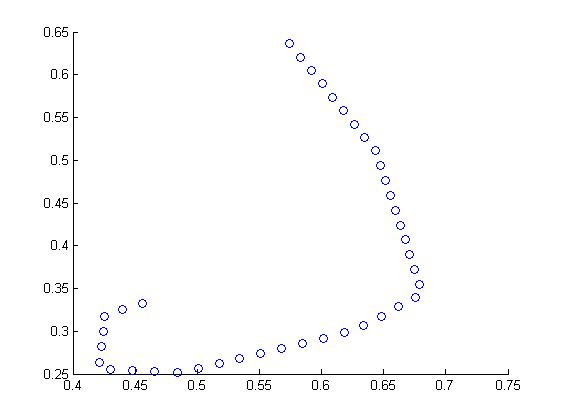
\includegraphics[width=0.5\textwidth]{./figures/letter_before_preprocessing}
        }
        \subfloat[]{
           \label{fig:letter_after_preprocessing}
           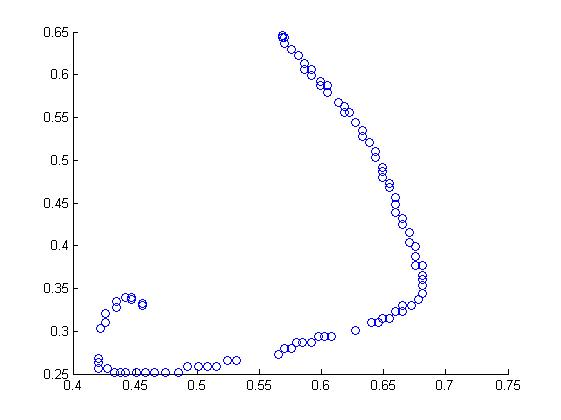
\includegraphics[width=0.5\textwidth]{./figures/letter_after_preprocessing}
        }        
    \caption{The letter \RL{d} before (a) and after (b) preprocessing}
   \label{fig:D_before_after_preprocessing}
\end{figure}

\emph{refer to the slant and Rotation normalization, i.e. why we don't do it. Is slant common in Arabic?
}

\subsection{Normalization and Translation}

Size normalization is done to achieve a uniform size of the bounding box surrounding the pattern. This is done to enable the classifier to recognize the sequence pattern even when the stroke is written in different sizes. Shape similarity algorithms tend to be sensitive for non-uniform shapes size, thus this procedure is important and can be found in many approaches in the literature. 
However, this method could not be applied since normalization is done in our system on the stroke level which could contain a letter, at least.
In our approach size normalization was applied on each stroke such that all strokes have $[0,1]\times[0,1]$ bounding box but retain their original aspect ratio. We include in this step also translation of the sequence's center of gravity to the origin point $[0,0]$.
Given the stroke sequence $S=\{p_i\}_{i=1}^{n}$, the normalized sequence $\bar{S}=\{\bar{p_i}\}_{i=1}^{n}$ is calculated by: 

\begin{equation}
{\bar x_i} = {{\left( {{x_i} - {\mu _x}} \right)} \over W},{\bar y_i} = {{\left( {{y_i} - {\mu _y}} \right)} \over W}
\end{equation}
Where
\begin{equation}
\mu  = \left( {{\mu _x},{\mu _y}} \right) = \left( {{1 \over N}\sum\limits_{i = 1}^N {{x_i}} ,{1 \over N}\sum\limits_{i = 1}^N {{y_i}} } \right)
\end{equation}
\begin{equation}
W = \max \left( {{d_x},{d_y}} \right)
\end{equation}
\begin{equation}
{d_x} = {x_{\max }} - {x_{\min }};\,\,\,{d_y} = {y_{\max }} - {y_{\min }}
\end{equation}
\begin{equation}
{x_{\max }} = \mathop {\max }\limits_i \left( {{x_i}} \right),\,\,{x_{\min }} = \mathop {\min }\limits_i \left( {{x_i}} \right),\,\,{y_{\min }} = \mathop {\min }\limits_i \left( {{y_i}} \right),\,\,{y_{\min }} = \mathop {\min }\limits_i \left( {{y_i}} \right)
\end{equation}  

\subsection{Noise Elimination}
The input obtained by the digitizer may contain a large amount of noise which is mainly duplication of points. In this process redundant points are filtered out and a similar sequence with fewer points is obtained.
In order to eliminate redundant points irrelevant for pattern classification and screening out unwanted noise and vibrations in the letter inscription we have used the \emph{Douglas-Peucker Polyline Simplification algorithm} described in \cite{douglas1973algorithms}. Briefly, it is a line simplification algorithm to reduce the number of vertices in a piecewise linear curve according to a specified tolerance. The algorithm is also known as \emph{Iterative Endpoint Fit}. The resulted curve is a skeletonized angular sequence. The Normalization is done before the Simplification, since we need a constant simplification parameter $\varepsilon$ which was tuned for $1\times1$ bounds. 
Assuming the stroke presentation is a sequence of points $S$, the sensitivity parameter that was used in our work is:
\begin{equation}
\varepsilon  = {1 \over {200}}\sqrt {{d_x}^2 + {d_y}^2}
\end{equation}

\begin{figure}
\centering
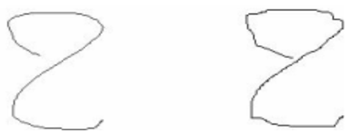
\includegraphics[width=0.7\textwidth]{./figures/ha_simplification}       
\caption{Non Simplified representation of the letter \RL{.h} (Ha) is shown on the right. A simplified version is shown on the left. \emph{TODO: change the pictures to something better}}
\label{fig:ha_simplification}
\end{figure}

\subsection{Smoothing and Re-sampling}
As a result of the simplification process the points are not distributed uniformly along the stroke trajectory. Naturally, there are less point in relatively straight areas and a higher amount of points in the curved areas of the stroke.\\ 
%if we wont use simplification we can write this: The re-sampling is needed to prevent the unbalanced sampling density, which may be influenced by the sampling rate and the user non-uniform letter drawing. 
The re-sampling produces equidistant smoothed data sequence. 
The Re-sampling is performed using splines interpolation as follows:\\
Given a stroke $S=\{p_i\}_{i=1}^{n}$ and the re-sampling target number $R$, let $\{X(a_i)\}_{i=1}^{n}$ and $\{Y(a_i)\}_{i=1}^{n}$ represent the x-axis and the y-axis sequences with respect to the parameter $a_i$ which is defined as follows:

\begin{equation}
a_i=a_{i-1}+arclen(p_{i-1},p_i) 
\end{equation}  

\begin{equation}
X(a_i)=x_i 
\end{equation}  

The arc-length of the stroke is given by $L=a_n$.\\

A piecewise linear interpolations $q_X(a)$ and $q_X(a)$ are created for the $X$ sequence and $Y$ sequence respectively.
The breaks are the $a_i$ sequence and the coefficient of the linear polynomial are $\alpha_{i} = \frac{X(a_i)-X(a_{i-1})}{a_{i}-a_{i-1}}$ 

\emph{[we use quadratic splines for smoothing and simplification.]}

let $t_i=i\frac{L}{R}$ for $i=0,...,R$.
The re-sampled sequence is given as follows:
\begin{equation}
\widehat{S}=\{(q_X(t_i),q_Y(t_i))\}_{i=1}^{R}
\end{equation}

The target number of points is set to 40. We had to find a number that is good enough for both long and short strokes since strokes can span over a single letter or a whole WP.

\emph{[TODO: show the following images: 1. the scattered stroke, 2. X and Y as a function of t., 3. X and Y resampledm and 3. the stroke resampled. ]}

\emph{[TODO: talk about splines.]}

\emph{TODO: talk about the other smoothing techniques as described in \cite{jaeger2001online} -- Online handwriting recognition: the NPen++ recognizer}

\subsubsection{Approach 1 - Using piecewise linear interpolations}

\subsubsection{Approach 2 - Using quadratic splines}

\begin{figure}
\centering
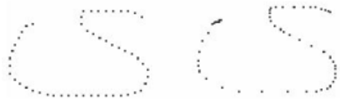
\includegraphics{./figures/y_resampling}       
\caption{Representation of a non-resamples sequence of the letter \RL{y} (Y) is shown in the right. The re-sampled version is shown on the left.}
\label{fig:y_resampling}
\end{figure}

\subsection{Implementation}
Answer the following:
\begin{itemize}
\item Mention that the data in the database was not in the same length and thus normalziation and re-sampling were needed. 
\item Where preprocessing is used in our system? Letters Learning and strokes classification
\item What parameters were used for each preprocessing stage and why.
\item what alternatives were considered.
\end{itemize}

%%%%%%%%%%%%%%%%%%%%%%%%%%%%%%%%%%%%%%%%%%%%%%%%%%%%%%%
\newpage{}
%%%%%%%%%%%%%%%%%%%%%%%%%%%%%%%%%%%%%%%%%%%%%%%%%%%%%%%

\section{Features Extraction}

Answer the following:
\begin{itemize}
\item Discussion - why did we decided to concentrate on shape context and MAD.
\item Discussion - Is combining several feature extraction technique is recommended?
\item Results - show the difference between MAD and SC.
\end{itemize}

Feature extraction is certainly one of the important parts of any pattern classification system. It aims is to cull informative parameters for learning and recognition of patterns.  Most classification methods require that patterns be represented in a fixed dimensional feature space that is often incompatible with input data. Poor feature extraction and selection will always result in a poor system performance, regardless of the ingeniousness of the learning and classification algorithms \cite{parizeau2001character}.\\

Feature extraction is commonly used in pattern recognition. While its goal is same in all fields, feature extraction methods operate differently in different domains. For instance, in the image retrieval field, the input data (i.e. the image) is too large and suspected to be redundant. In this case, feature extraction techniques are used to reduce the representation of the input data into a compact representation set of features. However, In the shape recognition domain, the input data is compact and feature extraction techniques are used to transform it into feature vectors, which are usually referred to as shape descriptors. Shape descriptors offer discriminative characterization to capture the perceptual dissimilarity between two shapes. Unlike in the first case, the raw quantity of data contained in feature vector usually exceeds the amount of data in the input data.\\

The goal of a shape descriptor is to be able to effectively find perceptually similar shapes from a database. Shape descriptors are usually in the form of vectors that are produced to represent a given shape feature and attempts to quantify perceptual similarities between shapes. That is to say, shapes which are found perceptually similar by human have resembling descriptor than from shapes that are different from the others. Effective shape descriptor must present some essential properties such as translation, rotation and scale invariance. It also must be as robust as possible against noise so that variously distorted shapes which are tolerated by human beings when comparing shapes. This is known as the robustness requirement.\cite{zhang2004review}\\

Low computation complexity is an important characteristic of a desirable shape descriptor. Efficiency of a descriptor is equally important as effectiveness due to the on-line retrieval demand. The descriptors should be represented and stored compactly. The size of a descriptor vector must not be too large. 

A shape descriptor is usually measured according to several principles which include good retrieval accuracy, compact features, low computation complexity and robust retrieval performance. \cite{kim2000region}

\emph{TODO: add a mathematical definition of the feature extraction as a transformation from the space domain to the feature space.}

Many shape description have been developed in order to improve the segmentation and recognition rates. There are many different classifications and sub classifications of shape descriptors according to their method of operation.The most common classification is the classification for local and global descriptors. Local descriptors calculate some feature at each sample point. Simple local features include the y coordinate and tangent slope angle. \emph{Normalized curvature} and \emph{Ratio of tangent} \cite{hu1995invariant,hu1996hmm} are examples of more complex local shape descriptor. Descriptors such as cusps, crossings and loops are referred to as global descriptors and are calculated on the entire shape \cite{hu1997combining}.

\emph{TODO: review "Local vs. global Features" (p. 30) in \cite{connell2000online} }

For a detailed review on shape descriptors see \cite{zhang2004review} and \cite{yang2008survey}.

Many well known and powerful features operate on the contour of the shape. This is because many descriptors were developed for off-line handwriting recognition in which the shape is the script contour. In the on-line handwriting recognition, the input data is a sequence of points  and no contour is involved, however using features in on-line handwriting recognition that we originally developed for the off-line case is common. Saabne and El-Sanna have used the \emph{Shape Context} (SC) descriptor, a global shape descriptor that was developed for contour based shapes, for the online handwriting recognition in \cite{saabni2009hierarchical}. Multi Scale shape context, a combination of three different shape contexts:
stroke, local neighborhood and global shape contexts, is used by Hu and Zanibbi in \cite{husegmenting} for on-line handwritten mathematical expressions segmentation.

In this work we have chosen to work with two shape descriptors, the Shape context descriptor and the tangent angle feature. The reason for this choice is that we wanted to investigate how both global and local features effectiveness in our proposed process. More information about these features are given in section \ref{sec:shape_context} and in section \ref{sec:mad}

In this work we have selected two features to work with, the Shape Context and the Multi Angular Descriptor. Generally, when considering shapes, the contour of the shape is taken into account, thus the following 2 shape descriptors is defined using the contour of the shape. However in the on-line writing recognition case, the features are applied upon the stroke sequence. 

\subsection{Shape Context}
\label{sec:shape_context}
\nomenclature{$SC$}{Shape Context Descriptor}
Belongie and Malik have presented a point matching approach named Shape Context \cite{belongie2002shape}. The Shape context is a shape matching approach that intended to be a way of describing shapes that allows for measuring shape similarity and the recovering of point correspondences. This approach is based on the following descriptor: Pick $n$ points on the shape's contour, for each point ${p_i}$ on the shape, consider the $n - 1$ other points and calculate the coarse histogram of the relative coordinates. Equation \ref{eq:sc_bins} is defined to be the shape context of ${p_i}$.

\begin{equation}
{h_i}(k) = \# \{q \ne p_i:(q - p_i) \in bin(k) \}
\label{eq:sc_bins}
\end{equation}

The bins are normally taken to be uniform log-polar space making the descriptor more sensitive to positions of nearby sample points than to those of points farther away. This distribution over relative positions is robust and compact, yet highly discriminative descriptor. The basic Idea of the Shape Context Descriptor is illustrated in Figure \ref{fig:shape_context_demo}. This can be calculated in $O(N^3)$ time using the Hungarian method. 

\emph{TODO: mention that the resulting is a histogram, and that there are many similarity measures methods that are good with histograms}

\begin{figure}
\centering
\subfloat[]{
    \label{fig:shape_context_offline}
    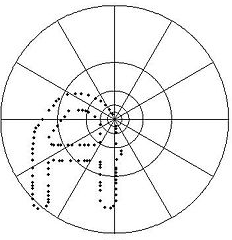
\includegraphics[width=0.27\textwidth]{./figures/shape_context_offline}
}
\subfloat[]{
	\label{fig:shape_context_online}
     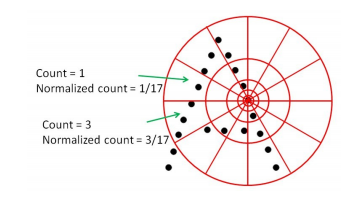
\includegraphics[width=0.5\textwidth]{./figures/shape_context_online}
}        
\caption{Diagram of the log-polar bins used to compute the shape context. On-line and off-line}
\label{fig:shape_context_demo}
\end{figure}

\subsection{Multi Angular Descriptor}
\label{sec:mad}
\nomenclature{MAD}{Multi Angular Descriptor}
The other shape descriptor used in this thesis is the Multi Angular Descriptor (MAD).
MAD was proposed by Saabni in \cite{saabni2013multi}. It captures the angular view to multi resolution rings in different heights. The shape is treated as a two dimensional set of points and the different rings are upper view points from rings around the shape centroid with different sizes and heights. To enables scale and translation invariance, the sizes and heights of these rings are calculated using the diameter and centroid of the shape.
Formally, let $S$ be a shape and Let $C$ and $D$ be the centroid and the diameter of the shape respectively. Let $P = \{p_i\}_{i = 1}^l$ a set of $l$ point taken uniformly from the extracted contour of $S$. Given a view point $V_j$ from a given ring with height $h$ over the shape, the angle, obtained by connecting the point ${p_i} \in P$ with each point   and the plain of the shape is a rich description of the shape from this view point. Let $R$ be a ring with the radius $r$ and the center $C$ positioned above the shape $S$ with the height $h$. Let $V = \{V_i\}_{i = 1}^n$ be a set of $n$ viewpoints lying uniformly on the ring $R$ and $\alpha(V_{ij})$ to be the angle between the segment $\overline {{V_i}{p_j}}$ and the plain contains the shape $S$. The vector $Ve{c_i} = \left\{ {\alpha \left( {{V_{ij}}} \right)} \right\}_{j = 1}^l$ can be seen as watching the shape $S$ from one upper view point $V_i$. Illustration can be seen in Figure 7.

\begin{figure}
\centering
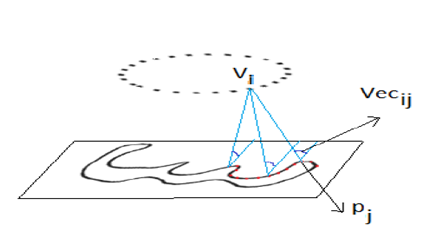
\includegraphics[width=0.7\textwidth]{./figures/mad_demo}       
\caption{In this figure we can see an example of three line segments drawn from the same viewpoint $V_i$, generating the three angles $Vec_{ij}$ with the plane of the shape. When the parameter $j$ goes over all contour points we get the vector $Vec_i$ describing the shape from the view point $V_i$ with the parameter $i$ goes over all viewpoints.}
\label{fig:mad_demo}
\end{figure}

\subsection{Implementation}

For each sample in the set, after preprocessing, one of the shape descriptors mentioned above was extracted. We 

Answer the following question:
\begin{itemize}
\item which results has achieved every method?
\item were there any implementation details we need to mention?
\item perform the following test - create a test set of letters and calculate the recognition rate for each shape descriptor.
\end{itemize}


%%%%%%%%%%%%%%%%%%%%%%%%%%%%%%%%%%%%%%%%%%%%%%%%%%%%%%%
\newpage{}
%%%%%%%%%%%%%%%%%%%%%%%%%%%%%%%%%%%%%%%%%%%%%%%%%%%%%%%

\section{Similarity Measure}

In this chapter we will discuss methods that were used in this work to asses the similarity measure between two handwritten curves. Identically, these method are usually used to compute dissimilarity between vectors in the features space. The dissimilarity degree between a feature of one shape to another feature of other shape often reveals how similar the two shapes are. 

Given two data inputs or feature vectors, we aim to define a quantitative measure of their dissimilarity with the intent of approximating perceptual resemblance between them. The task of mathematically capturing the human perceptual shape differences is not an easy task. A good similarity measure should be able to cope with various types of discrepancy, such as shifting, noise and scaling. Such variations can be easily handled by a human. Time shifting may be caused by different sampling rate, and noise may be introduced by sensor failures, errors in detection techniques, and disturbance signals \cite{chen2005similarity}. 

The similarity measure is needed to answer the following query: 
Given a objects database DB and a query object q, find all objects in DB that are perceptively similar to q. Thus, it has a direct and crucial affect on the matching quality of the classification results. 

\emph{show a picture from the DTW or from the thesis that demonstrates the problem with similarity measure.}

The similarity measure is formalized as a so-called distance function. 

\begin{definition}
Given a space $D$, as defined in section \ref{[]}. For any two data elements $x,y \in D$, a \emph{distance function}, dist, on $D$ is defined as:
\begin{equation}
dist: D \times D \longrightarrow \mathbb{R}
\end{equation}
where $\mathbb{R}$ is the real data set and $dist$ has the following properties:
\begin{itemize}
\item $dist(x,y)=0 \Leftrightarrow x=y$ (reflexivity)
\item $dist(x,y) = dist(y,x)$ (symmetry)
\end{itemize}
The pair $(D,dist)$ is called a distance space.
\end{definition}

The distance function depends on the application and the data representation and needs to be carefully designed to fit the problem domain. Significant amount of research has been carried out on similarity measure functions, both in distance functions and their efficient evaluation. 
Much of the previous research was done on similarity search over time series and distributions. 

Under the definition of a distance function, a formal definition of the query mentioned earlier ,namely the \emph{range query}, can be given as follows: 
For a given distance function $dist$, a query object $q$ and a search radius $r$, return all sample objects that fall within $r$ distant from $q$, i.e. $dist(q,x) \leq r$. See figure  \ref{fig:range_query}.

Other types of queries are discussed in the literature, most notably the \emph{nearest neighbors query}, which "" returning all the closest sample (or k samples) objects to the query object. It can be argued that range queries are fundamental, and virtually all published metric indexing methods support them \cite{hetland2009basic}.

\begin{figure}
\centering
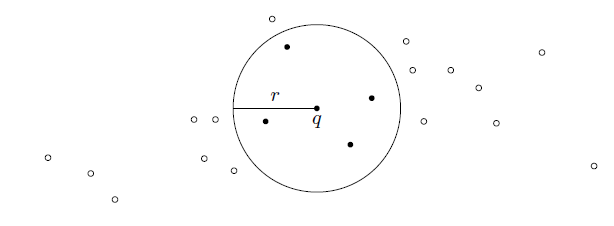
\includegraphics[width=0.7\textwidth]{./figures/range_query}       
\caption{Visualization of a range query in two-dimensional Euclidean space. The small circles are objects in the data set, while the filled dots are returned as a result of the query with sample object $q$ and search radius $r$}
\label{fig:range_query}
\end{figure}

\begin{definition}
$L_p$-norm: Given two sequences $R$ and $S$ of the same length $N$, the $L_p$ norm distance between $R$ and $S$ is:
\begin{equation}
L_p-norm(R,S)=\sqrt[p]{\sum\limits_{i=1}^N d(r_i,s_i)^p}
\end{equation}
Where $d(r_i,s_i)$ is the distance function between $r_i$ and $s_i$. 
\end{definition}
$L_1-norm$ is called the \emph{Manhattan distance} or \emph{city block distance}, $L_2-norm$ is known as the \emph{Euclidean distance}.

$d(r_i,s_i)$ is also a matter of choice. However, in most cases it is defined as the $L_2-norm$, i.e. 
\begin{equation}
d(r_i,s_i)=\sqrt[2]{({r_{i_x}-s_{i_x}})^2+({r_{i_y}-s_{i_y}})^2}
\end{equation}

Euclidean distance is the most basic distance function, it is easy to compute and the computation cost is linear in the sequence length.

However, the Euclidean distance has some disadvantages in regards to curve sequences. First, it requires the two sequences to be of the same length. Second, it does not support local shifting. 
Local shifting occurs when one point of one sequence is shifted  to match an element of the another sequence (even when the two matched elements appear in different positions in the sequences). It is important when the compared sequences have similar shape but are out of phase. It is called "local", because not all of the points of one sequence need to be shifted in the same factor and direction to match the other sequence. By contrast, in "global" shifting, all the points are shifted along the same direction by a fixed shifting factor. Generally, local time shifting cannot be handled by $L_p-norm$, because it requires the $i^{th}$ element of query sequence be aligned with the $i^{th}$ element of the data sequence \cite{chen2005similarity}. 
The Euclidean distance function is a \emph{metric}. A formal definition of a metric is given below. (Defenition \ref{def:metric})

\begin{definition}
Given a data space $D$. A distance function $dist$ is a \emph{metric} if for all $x,y,z \in D$, the following two additional conditions hold:
\begin{itemize}
\item $dist(x,y)=0 \Leftrightarrow x=y$ (reflexivity)
\item $dist(x,z) \leq dist(x,y) + dist(y,z)$ (triangle inequality) 
\end{itemize}
In this case, the pair $(D,dist)$ is called \emph{metric space}.
\label{def:metric}
\end{definition}

Mathematically, metric spaces are a generalization of Euclidean space, keeping some of its well-known geometric properties. These convenient properties allow us to achieve more efficient data structures and search algorithms. 

The most important property of a metric function is triangle inequality since most of the indexing structures assume that the underlying distance functions follow triangle inequality. One way of interpreting triangularity is that the concept of overlap becomes meaningful for naturally defined regions such as metric balls. If we're allowed to violate triangularity, two seemingly non-overlapping balls could still share objects. See figure \ref{fig:non_triangular_space} \cite{chen2005similarity}.

A second aspect related to similarity-based retrieval is how to improve retrieval efficiency. The execution time is of a query mainly affected by the number of distance computations. The triangularity property facilitate fast retrieval by using indexing and lower bounding. This aspect will be discussed in details in section \ref{[]}.

The idea of using triangle inequality for Indexing will be discussed in the next chapter.

\begin{figure}
\centering
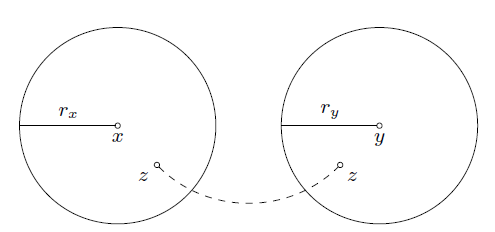
\includegraphics[width=0.7\textwidth]{./figures/non_triangular_space}       
\caption{Illustration of a non-triangular space. Two regions defined as balls (everything within a distance rx and ry of x and y, respectively) seemingly don't overlap, as d(x, y) > rx + ry. Even so, there may be objects (such as z) that are found in both regions}
\label{fig:non_triangular_space}
\end{figure}

{\color{blue}Distance functions have been proposed for different application, such as Dynamic Time Warping [12, 118, 57, 52], Longest Common Subsequences [13, 108], Edit distance. 
Dynamic Time Warping (DTW), which will be described in details in section \ref{[]}, can handle sequences with different lengths and local time shifting, but it does not follow triangle inequality, which is one of important properties of a metric distance function. Furthermore, Euclidean distance and DTW are sensitive to noise, thus, they are not suitable for data that contain noise. Longest Common Subsequence (LCSS) is proposed to handle possible noise that may appear in data; however, it ignores the various gaps in between similar subsequences, which leads to inaccuracies. \cite{chen2005similarity}.}

Indexing techniques of measure functions is not fast enough to our approach strict requirements. Thus we still need to use the euclidean space and integrating sub-linear search technique to achieve the needed performance and also we can't afford performing the computations the similarity measures mentioned above even if the number of computation is sub-linear. Thus we have taken a different approach and used embedding technique to facilitate using 

\subsection{The Earth Movers Distance}

\emph{Earth Movers Distance} (EMD), introduced by Rubner et al. in \cite{rubner2000earth}, is a measure of the dissimilarity between two histograms. It has experimentally verified to capture well perceptual notion of a difference between images \cite{grauman2004fast}, since, Images are usually represented using multidimensional histograms. In fact, it is widely used in content-based image retrieval to compute distances between the color histograms of two digital images \emph{TODO: and citation}. 

Histogram based descriptors, such as shape context, are usually compared using bin-wise dissimilarity measure like $L_2$ norm or the $\chi^2$ statistic. While these measures can be computed very fast, since they measure dissimilarities between the content of corresponding bins of the two histograms, they usually fail to consider local and global variations. These um-modeled variations may result in large dissimilarity values between two histograms that are perceived to be small.

Generally speaking, the distance between two histograms is a special case of the well-known \emph{transportation problem}, a.k.a the Monge-Kantorovich problem \cite{rachev1985monge} defined below (Definition \ref{def:transportation_problem}). Accordingly, EMD is based on the solution to the transportation problem, for which efficient algorithms are available. 

\begin{definition}
\label{def:transportation_problem}
Given several \emph{suppliers} and \emph{consumers}. Each supplier, $P_i$, having a given amount of goods $p_i$, and each consumer, $Q_j$, having a given amount of demand, $q_j$. For each supplier-consumer pair, the cost of transporting a single unit of goods is given, $d_{ij}$. The transportation problem is then to find the a least expensive flow of goods from supplier to consumer that satisfies the consumer's demand, i.e., finding the flow $f_{ij}$ between $P_i$ and $Q_j$ which minimizes:
\begin{equation}
COST(P,Q,F)=\sum\limits_{i=1}^{m} \sum\limits_{j=1}^{n} d_{ij}f_{ij} 
\end{equation}
subject to the following constrains:
\begin{equation}
f_{ij} \geq 0, 1\leq i \leq m, 1\leq j \leq n 
\end{equation}
\begin{equation}
\sum\limits_{j=1}^{n} f_{ij} \leq p_i, \forall 1\leq i \leq m
\end{equation}
\begin{equation}
\sum\limits_{i=1}^{m} f_{ij} \leq q_j, \forall 1\leq j \leq n
\end{equation}
\begin{equation}
\sum\limits_{i=1}^{m} \sum\limits_{j=1}^{n} f_{ij} = \min\left( \sum\limits_{j=1}^{n} f_{ij} \leq p_i, \sum\limits_{i=1}^{m} f_{ij} \leq q_i \right)
\end{equation}
\end{definition}

In the case where the total amount of goods equals the total amount of goods demanded, the solution is a complete one-to-one correspondence. i.e. given a matching function $pi:Q \rightarrow F$,
\begin{equation}
 COST(Q,F)=\min_{\pi:Q \rightarrow F} \sum_{p_i \in P} D(p_i,\pi(p_i))
\end{equation} 

Once the general transportation problem solved, and optimal flow $f$ was found, EMD is defined as the cost normalized by the total flow. A formal definition of EMD metric is given as follows:

\begin{definition}
Given two histograms $h, g$, a ground distance $d_{ij} \geq 0$ and a flow $f_{ij} \geq 0$ (from bin $h_i$ to bin $g_j$). EMD is defined as follows:
\begin{equation}
EMD(h,g)=\min{\frac{\sum_{i,j} f_{ij}d_{ij}}{\sum_{i,j} g_{ij}}}
\end{equation} 
such that $\sum_{j} f_{ij} \leq h(i)$, $\sum_{i} f_{ij} \leq g_i$, $\sum_{i,j} f_{ij}=min\left(\sum_{i} h_i, \sum_{i} g_i\right)$
\end{definition}

EMD is a natural and intuitive metric. Descriptively, if the histograms are interpreted as two different ways of piling up a certain amount of sand, the EMD is the minimal cost of turning one pile to other. EMD is the minimal total ground distance traveled, weighted by the amount of sand moved (called flow). When used to compare histograms with the same overall mass, EMD is a metric.

{EMD being a transportation problem, can also be modeled as a network flow problem in graph theory. The two histograms are represented by a single graph with a vertex for each bun and a graph distance as the edge weights. The two histogram vertices act as sources abs siinks respectively with bin content as values. Computing EMD is now an uncapacitated minimum cost flow problem and can be solved by Orlin's algorithm in $O(N^3 logN)$\cite{}}

As seen in previous sections, Both features used in this thesis produces histograms. The implementation used in this work for the SC produces a feature vector with a constant total mass. In this case, EMD is a true metric and thus it is the the best fit for our needs.

EMD was used by Saabne in \cite{[]} for off-line handwriting recognition. However, for the best of our knowledge, this is the first use of EMD in the on-line handwriting recognition. {TODO: give more examples of usages, be more specific about the handwriting recognition field.} 

The major hurdle to using EMD is its $O\left( {{N^3}\log N} \right)$ computational complexity (for an N-bin histogram). The complexity is magnified when the task is to search for similar shapes (nearest neighbors) in a large database. In this case, a linear scan of the database would require computing a comparison of superpolynomial complexity for each database member against the query shape. Hierarchical search methods, pruning, or the triangle inequality may be employed, yet query times are still linear in the worst case, and individual comparisons maintain their high complexity regardless.\cite{grauman2004fast}.

In the next subsection, we will discuss an EMD embedding technique which spares the linear scan of the entire database and greatly reduce the computation effort in approximating the EMD distance between two objects.

%%%%%%%%%%%%%%%%%%%%%%%%%%%%%%%%%%%%%%%%%%%%%%%%%%%%%%%
\newpage{}
%%%%%%%%%%%%%%%%%%%%%%%%%%%%%%%%%%%%%%%%%%%%%%%%%%%%%%%

\section{Nearest Neighbors Retrieval}

\underline{Mind Map:}
\begin{enumerate}
\item problem definition.  \cite{hetland2009basic}
\item The L-p norm has an advantages and drawback.
\begin {itemize}
\item calculates fast and it is a norm
\item bin-ton-bin correspondence thus do not handle local deformations
\end {itemize} 
\item complicated dissimilarity function has also advantages and drawbacks.
\begin {itemize}
\item they are better at capturing the dissimilarity.
\item But are very expensive to calculate.
\item and also are not norms, thus fast retrieval data-structures can't be used.
\end {itemize} 
\item pruning and indexing can be used to spare calculations. \cite{chen2005similarity}
\begin {itemize}
\item what is pruning and what properties are needed for it.
\item what is indexing and what properties are needed.
\item Why it is not good for us.
\end {itemize}
\item EMD embedding
\begin {itemize}
\item Embedding by Indyk. (what is the exact setup, what are the bounds)
\item Krishnan paper - what does he bring to the discussion? 
\item Approximate Embedding by Shirdhonkar. (what is the exact setup, what are the bounds)
\end {itemize}
\item fast retrieval algorithms on normed spaces
\begin {itemize}
\item give an introduction, mentiond kdtree, Rtree and LSH (each one with its advantages and drawbacks)
\item kd-tree.
\end {itemize}
\item compare SC and MAD and angular, contour results under the embedding.
\end{enumerate}

Answer the following:
\begin{itemize}
\item How is the classification is done - mention that the system recieves a stroke and it goes over all the stages
\item A list of candidates is retrieved by the kdtree, then to be more precise we use a combination of the Constrained DTW metric and the distance of the sample and the candidate.
\item mention the alternatives - using different combination (we can afford using heavy tools since we have small candidate number)
\item we return the best 3 candidates.
\end{itemize}

As been said before, an important question is how to build a data-structure that quickly identifies the objects that are closest to a query object (the nearest neighbor search problem).

For the reader convenience and for the sake of completeness, first we would like to give the definition of \emph{normed vector space}.

\begin{definition}
Given a vector space $D$ over a field $F$ the pair $\left(D,\|\cdot\|\right)$ is a \emph{normed space}, if for all $x,y\in D$ and $\alpha \in F$ the following conditions hold:
\begin{itemize}
\item $\|x\|=0 \Leftrightarrow x=0$
\item $\|x-y\| \geq|\|x\|-\|y\||$
\item $\|\alpha x\|=|\alpha\|x\|$
\end{itemize}
\end{definition}

Using normed spaces such as $L_p-norm$ to solve the dissimilarity measure problem has the advantage that in order to solve the nearest neighbor problem, one can use data structures, such as kd-trees and R-trees, which are specifically designed for points living in the normed space. Such data structures provide mechanisms for answering the NN-query that are orders of magnitude faster than linear scan of the database. However, the quality of the dissimilarity measure of such norms is not always satisfactory \cite{indyk2003fast}.

On one hand, we would like to use advanced similarity measure technique that corresponds to the human intuition. These distance measure techniques are usually require high complexity time and also are not metrics. On the other hand, we need to be able efficiently compute the distance measure between two objects and also not have to search linearly the entire database in-order to get the most similar objects in the sample set.

In this chapter we will discuss the usage of pruning and indexing techniques and consider the advantages and drawbacks. We will also consider an embedding techniques that allows us to get the best of the both fast similarity measure calculation and use the advantages of the normed space. It will allow us to approximate the EMD distance between two histograms, and since the embedding is into an $L_1$ normed space, efficient object retrieval data structures can be used. 


\subsection {Appendix - Indexing and Pruning Techniques}

{\color{blue}Index structures are structures built over the given data set in order to speed up queries. The time cost involved in building the index is amortized over the series of queries, and is usually ignored when considering search cost. The main goal, then, of an index method is to enable efficient search, either asymptotically or simply in real wall-clock time.\cite{hetland2009basic}}

{\color{blue}Similarity search is a mode of information retrieval where the query is a sample object, and the desired result is a set of objects deemed to be similar - in some sense - to the query.
Under the distance function formalism, several query types may be formulated. In the following I focus on one of the basic kinds, so-called range queries, where all objects that fall within a given distance of the sample are returned. In other words, for a distance function $dist$, a query object $q$, and a
search radius $r$, objects x for which $dist(q, x) \leq r$ are returned. Another type of query is the nearest neighbors query (returning the nearest object, or the k nearest objects)
It can be argued that range queries are fundamental, and virtually all published metric indexing methods support them. \cite{hetland2009basic}}.

{\color{blue}The idea of using triangle inequality to remove false candidates is illustrated. A distance function dist defined on a data space D satisfies triangle inequality, if and only if 
\begin{equation}
\forall Q,R,S \in D, dist(Q,S)+dist(R,S) \geq dist(Q,R)
\end{equation}
By rewriting inequality 2.9, $dist(Q,S) \geq dist(Q,R) - dist(R,S)$ can be derived. If $dist(Q,R)$ and $dist(R,S)$ are known, $dist(Q,R) - dist(R,S)$ can be treated as a lower bound distance of dist(Q,S). If the current query range is $r$ and $dist(Q,R)-dist(S,R)> r$, the computation of dist(Q,S) can be saved since S does not belong to the answer set. This is the basic principle that most of distance-based indexing structures follow.\cite{chen2005similarity}}


\subsection{Approximating EMD using Embedding}

Various approximation algorithms have been proposed to speed up the computation of EMD \emph{TODO: add refernces}. Indyk and Thaper, in \cite{indyk2003fast}, has suggested an embedding technique in which the un-normed EMD metric is embedded into a normed space, so that the distance between the two images is comparable to the distance between the two points which represent the embedding of the two images. Embedding time complexity is $O(Nd log{\Delta}$, where $N$ is the feature set size, $d$ is the feature space dimension and $\Delta$ is the diameter of the union if the two feature sets.

The embedding of EMD provides a way to map weighted point sets $A$ and $B$ from the metric space into the normed space $L_1$, such that the $L_1$ distance between the resulting embedded vectors is comparable to the EMD distance between $A$ and $B$. The motivation of doing so is that the working with normed space is desirable to enable fast approximate Nearest Neighbors (NN) search techniques such as LSH and kdTree. 

A brief description of the embedding technique proposed by Indyk:
{\color{blue}The embedding of EMD given in \cite{indyk2003fast} provides a way to map weighted point sets A and B from the metric space into the normed space L1, such that the L1 distance between the resulting embedded vectors is comparable to the EMD distance between A and B themselves. Working in a normed space is desirable since fast approximate NN search techniques such as LSH require it. The general idea of the embedding is to compute and concatenate several weighted histograms of decreasing resolution for a given point set. Formally, given two point sets A and B, each of cardinality n, and each containing points in $R^d$: impose grids $G_i$, $-1 \leq i \leq log(\Delta)$, on the space $R^d$, with grid $G_i$ having side length $2^i$, and $\Delta$ equal to the diameter of $A \bigcup B$. Each grid is translated by a vector chosen randomly from $[0, \Delta]^d$. To embed point set A, for each $G_i$ create vector $v_i$ with one coordinate per grid cell, where each coordinate counts the number of points in the corresponding cell, i.e., each $v_i$ forms a histogram of A. The embedding of A is then the concatenated vector of the $v_i$'s, scaled by the side lengths:
$f(A) = [v_{-1}(A), v_0(A), 2v_1(A), . . . , 2^iv_i(A), . . .]$. The distortion of the embedding has an upper bound of $O(log \Delta))$ . See \cite{indyk2003fast} for details. The distortion $C$ of a metric embedding $f$ describes how much information loss the embedding induces: $\frac{1}{C}EMD(A,B) \leq \|f(A) - f(B)\|_{L_1} \leq EMD(A,B).$}

In the original work on EMD, the authors provided more general definition of EMD which does nor assume $|P|=|Q|$. However, Indyk did not consider this generalization, since in such case EMD does not form a metric. Indyk and Thaper do not prove this for individual random embeddings, and also do not estimate the constants that bound the ratio of the norm to EMD.

A work conducted by Shirdhonkar and Jacobs in \cite{shirdhonkar2008approximate} has proposed a method for approximating the EMD between two low dimensional histograms using the weighted wavelet coefficients of the difference histogram. The approximation is done by transforming the histograms to $L_1$ space so that the distance between the two vectors in the wavelet domain is the EMD approximation. They have proven the ratio of EMD to wavelet EMD is bounded by constants. The wavelet EMD metric can be computed in $O\left( N \right)$ time complexity.

\emph{give more details about the work done by Shirdhonkar. What are the estimates for the bound?. What coefficient was used and why? Is the approximation technique described by Shirdhonkar and Jacobs is applicable for different mass histograms? see works that referenced Shirdhonkar and Jacobs.}

In our framework, sub-strokes classification is done by finding a stored letter sample that is maximally similar to the shape of the sub-stroke.

For a given sub-stroke, we need to find the most perceptually close object in the sample set. Since our samples space is in $L_1$ we use NN classification method.

{\color{blue}To reduce the search space,we apply a series of filters in a hierarchical manner. The earlier filters perform light processing on a large number of candi- dates, and the later filters perform heavy processing on a small number of candidates. In the first filter, global fea- tures and delayed strokes patterns are used to reduce can- didate word-part models. In the second filter, local features are used to guide a dynamic time warping (DTW) classifi- cation. The resulting k top ranked candidates are sent for shape-context based classifier, which determines the recog- nized word-part. In this work, we have modified the classic DTW to enable different costs for the different operations and control their behavior\cite{saabni2009hierarchical}}

{\color{blue}There are drawbacks to using the simple positional feature for shape matching with approximate EMD.Though straight forward to embed, it can be a brittle feature, and in order to achieve scale or translation invariance this feature demand preprocessing stage on all shapes. \cite{grauman2004fast}}

\subsection{Nearest Neighbors search}

\underline{Mind Map}
\begin{enumerate}
\item Introduction - What is ANN?
\item How Expensive is the exact NN? What is the motivation to use ANN?
\item How good is the approximation?
\item pruning and indexing - from the thesis.
\item kd-tree -  is it an ANN or exact data-structure? what is the approximation parameter? is it only for the Euclidean norm? norm or metric?
\item In case of general metric space branch and bound approach is known under the name of metric trees. Particular examples include vp-tree and BK-tree.
\item note that LSH require only a metric space.

\end{enumerate}

After performing dimensionality reduction techniques on the letters samples, the samples are used to create a kdtree data structure to facilitate fast nearest neighbor retrieval.

In the \emph{k Nearest Neighbor} (k-NN) problem a set of data points in d-dimensional space is given and for a query point q, the nearest or generally k nearest points of P to q can be reported efficiently. The distance between two points can be defined in many ways as was details in section \ref{[]}.
 algorithm is a very basic common approach for implementing the pattern classification. However, the retrieval of the exact k-Nearest Neighbors for a given query object $q$ and a database of sample set $S$ suffers from bad performance that is mainly caused by two factors. The first, is the total numbers of samples in the data and the other is the dimensionality of objects in the data (known as the \emph{curse of dimensionality}). Computing exact nearest neighbors in dimensions much higher than 8 seems to be a very difficult task. However, the first issue has much smaller impact on the speed of the nearest neighbor retrieval and can be healed easily by using dimensionality reduction techniques. however, the first, i.e. the size of the sample data, is crucial. \\

The simplest solution to the NN problem is to linearly go over the entire sample set and keep track of the best k best nominates so far. The running time of this algorithm in $O(Nd)$ where $N$ is the cardinality of sample set and d is the dimensionality of the sample set. While looking in the entire database for the kNN is not permissible for most applications. The only advantage of this approach is that it requires no extra space, beyond the amount of the memory needed for keeping the sample set.

Many methods were proposed to solve the kNN problem that are significantly better than a brute-force computation the distances of the entire database. However, computing nearest neighbors approximately, can to achieve significantly faster with a relatively small actual errors. \emph{Approximate nearest neighbor} (ANN) techniques allows the user to specify a maximum approximation error bound, thus enabling the user to control the trade-off between accuracy and running time. It is usually done by preprocessing the data points and into a data-structure. \\

ANN methods such as k-d trees and Locality Sensitive Hashing (LSH) have successfully applied on variety of fast similarity retrieval problems. Unfortunately, the key assumption in these procedures is that objects in the dataset lie in a metric space. As mentioned in chapter \ref{}, this assumption is not valid for many similarity measure techniques. The disadvantage of the ANN is that a large portion of these techniques requires the classified objects to reside inside a normed space. Kd-tree requires a more specific $L_p$ metric space to operate in. 

\emph{TODO: give a small introduction on LSH in 1 or two sentences}


The advantage of LSH is that it operates way better than kdtree in a high dimensional space. However, the strength of kdtree is that it can be used as an exact NN technique. While the the worst case scenario complexity is $O(N)$, the expected complexity is $O(log N)$ 

\subsubsection{kd tree}
\underline{Mind Map}
\begin{enumerate}
\item a short introduction to kdtree
\item what is the complexity of building and searching in kdtree.
\item what flavour of kdtree did we use?
\item what is the approximation parameters of the kdtree.
\item who usually use this method? In what area/disciplines?
\item why did we chose kdtree and not LSH. 
\item in how much did it boost our performance when we used kdtree than id we had used exhaustive search?
\item mention that we use Matlab library kdtree implementation and talk about the bucket size. 
 \end{enumerate} 

{\color{blue}A kd-tree is a data structure for storing a finite set of points from a k-dimensional space. It was examined in detail by J Bentley. Recently S Omohundro has recommended it in a survey of possible techniques to increase the speed of neural network learning [Omohundro,1987]}

k dimensional tree (kd-tree), a special case of binary space partitioning trees, was proposed by Bentley in \cite{bentley1975multidimensional}. It aims at solving the problem of searching kNN in a large set of multi-dimensional points by first building a data structure based on the set of reference points. Then, given a query object, it extract the kNN using this structure.

{\color{blue}Every non-leaf node can be thought of as implicitly generating a splitting hyperplane that divides the space into two parts, known as half-spaces. Points to the left of this hyperplane are represented by the left subtree of that node and points right of the hyperplane are represented by the right subtree. The hyperplane direction is chosen in the following way: every node in the tree is associated with one of the k-dimensions, with the hyperplane perpendicular to that dimension's axis. So, for example, if for a particular split the "x" axis is chosen, all points in the subtree with a smaller "x" value than the node will appear in the left subtree and all points with larger "x" value will be in the right subtree. In such a case, the hyperplane would be set by the x-value of the point, and its normal would be the unit x-axis -- wikipedia kdtree}



\section{Clustering}
\begin{itemize}
\item Talk about the clustering process.
\item try to implement the number of clusters recommendation system.
\subsection{L1 K-medoids}
\end{itemize}

%%%%%%%%%%%%%%%%%%%%%%%%%%%%%%%%%%%%%%%%%%%%%%%%%%%%%%%
\newpage{}
%%%%%%%%%%%%%%%%%%%%%%%%%%%%%%%%%%%%%%%%%%%%%%%%%%%%%%%

\section{Features Transformation and Dimensionality Reduction}

Answer the following:
\begin{itemize}
\item what is DR and what is its important properties?
\item why do we need DR?
\item what type of DR are there - kernel based, bla bla bla?
\item why did we have choosen to use this DR although we are working in $L_1$ and PCA and LDA word in $L_2$?
\item what package we had used to try different DR techniques?
\item why did we combine LDA and PCA?
\end{itemize}


{\color{blue} Thus, instead of attaching a raw, full-dimensional shape context feature to each sampled object point, we use PCA to find a low-dimensional subspace based on a large sample of the shape context histogram. This sample is drawn from the database of contours on which we wish to apply our method. PCA yields the set of bases that define a low-dimensional "shape context manifold" All contours (database and novel queries alike) are then projected onto the subspace, and the approximate EMD embedding is performed in the domain of small number of their subspace.\cite{grauman2004fast}}

{\color{blue}When performing analysis of complex data one of the major problems stems from the number of variables involved. Analysis with a large number of variables generally requires a large amount of memory and computation power or a classification algorithm which overfits the training sample and generalizes poorly to new samples. Feature extraction is a general term for methods of constructing combinations of the variables to get around these problems while still describing the data with sufficient accuracy. (Word base line detection in handwritten text recognition systems -- Kamil R. Aida-zade and Jamaladdin Z. Hasanov)}

Feature transformation is a group of methods that create new features (predictor variables). The methods are useful for dimension reduction when the transformed features have a descriptive power that is more easily ordered than the original features. There are 2 main approaches for this task. One is \emph{feature selection} and the other is \emph{feature transformation}. 

Dimensionality Reduction is a process of reducing the number of random variables taken into consideration in the learning and classification of Data. Ideally, the reduced representation should have a dimensionality that corresponds to the intrinsic dimensionality of the data. Reducing the dimensionality of the features vectors would not only simplify and rapid the learning and classification task but rather boosts the classification accuracy.  Feature transformation technique is much more suitable to be implemented in our approach. In this work we have chosen to use two techniques applied in sequential manner in order to obtain the most efficient and linearly discriminative components, \emph{Principle Component Analysis} (PCA) and \emph{Linear Discrimination Analysis} (LDA) Technique. 

\subsection{Principle Component Analysis}
PCA was invented in 1901 by Karl Pearson. It is a linear technique for dimensionality reduction, which means that it performs dimensionality reduction by embedding the data into a linear subspace of lower dimensionality. Although there exist various techniques to do so, PCA is by far the most popular (unsupervised) linear technique. PCA is an orthogonal linear transformation that transforms the data to a new coordinate system such that the greatest variance by any projection of the data comes to lie on the first coordinate (names the first principal component), the second greatest variance on the second coordinate, and so on. Each principal component is a linear combination of the original variables. All the principal components are orthogonal to each other, so there is no redundant information. The principal components as a whole form an orthogonal basis for the space of the data.
The full set of principal components is as large as the original set of variables. But taking the first few principal components will preserve most of the information in the data, and reduces the data dimensions.

\subsection{Linear Discriminant Analysis}
PCA is an unsupervised technique and as such does not include label information of the data. The following example demonstrates the problem drawback: Imagine 2 cigar like clusters in 2 dimensions, one cigar has $y = 1$ and the other $y = -1$. The cigars are positioned in parallel and very closely together, such that the variance in the total data-set, ignoring the labels, is in the direction of the cigars. For classification, this would be a terrible projection, because all labels get evenly mixed and we destroy the useful information. A much more useful projection is orthogonal to the cigars, i.e. in the direction of least overall variance, which would perfectly separate the data-cases.

LDA is closely related to PCA in that they both look for linear combination of variables which best explain the data. LDA explicitly attempts to model the difference between the classes of data. In this method, variability among the feature vectors of the same class is minimized and the variability among the feature vectors of different classes is maximized.

The LDA performs dimensionality reduction while preserving as much of the class discriminatory information as possible. Without going into the math, in order to find a good projection vector, we need to define a measure of separation between the projections. The solution proposed by Fisher is to maximize a function that represents the difference between the means, normalized by a measure of the within-class scatter.

Although, LDA assumes that the distribution of samples in each class is Gaussian and that we cannot prove that the handwritten letters are distributes in a Gaussian manner, we selected LDA as 

Even though LDA is preferred in many application of dimension reduction, it does not always outperform PCA. In order to optimize discrimination performance in a more generative way, a hybrid dimension reduction model combining PCA and LDA is used in this work. 

\subsection{Implementation Details and Discussion}

In this system, we use a flavor the dimensionality reduction process can be outlines as follows: the pre-processed feature matrix $M$ projected into subspace $S_1$ using PCA and then into the subspace $S2$ using LDA. In the PCA stage, the largest $t$ eigenvalues are selected to create the PCA projection matrix $W_{PCA}$. $t$ is the number of eigenvalues which guarantee energy E is greater than 0.99. The data preservation value is calculates as seen in Equation \ref{eq:dr_energy} where ${\lambda _i}$ is the ith eigenvalue

\begin{equation}
E = {{\sum\limits_{i = 1}^t {{\lambda _i}} } \mathord{\left/
 {\vphantom {{\sum\limits_{i = 1}^t {{\lambda _i}} } {\sum\limits_{i = 1}^{\dim \left( S \right)} {{\lambda _i}} }}} \right.
 \kern-\nulldelimiterspace} {\sum\limits_{i = 1}^{\dim \left( S \right)} {{\lambda _i}} }}
\label{eq:dr_energy}
\end{equation}

The dimensionality of $W_{PCA}$ is much smaller that the dimensionality of $M$. At the second phase LDA is used to project $W_{PCA}$ to $W_{PCA+LDA}$.  The dimension of subspace $S_2$ is smaller than the subspace $S_1$ by 1.
Why we have used both and what give us every method and how we did join them together to get the most out of both.

\emph{Why we have used both and what give us every method and how we did join them together to get the most out of both.}

\emph{ Talk about other Dimensionality reduction techniques such as LMNN and show results.}


%%%%%%%%%%%%%%%%%%%%%%%%%%%%%%%%%%%%%%%%%%%%%%%%%%%%%%%
\newpage{}
%%%%%%%%%%%%%%%%%%%%%%%%%%%%%%%%%%%%%%%%%%%%%%%%%%%%%%%

 
\section{Letters Classification and Candidates Scoring}

\subsection{Data Time Warping}
\emph{Copy and paste from methods.docx} 
\end{document}
